
\subsubsection*{Methodology of the CALREC project}

%4. El detalle de la metodología propuesta en cada uno de los subproyectos participantes, incluyendo la viabilidad metodológica de las tareas. Si fuera necesario, también se incluirá una evaluación crítica de las posibles dificultades de un objetivo específico y un plan de contingencia para resolverlas.
%

{\bf Calibration of SiPMs and PMTs sensors}

The gain and noise of the PMTs and SiPMs sensors will be calibrated with 400 nm LEDs located on the tracking and energy plane. Each SiPM board has a place for one LED.
Calibration data will be acquired during the physics runs.
%During the physics runs, the LEDs will illuminate the chamber at small rate.
The gain and noise will be obtained from a fit to the single photo-electron spectrum.
They will be monitored along time and temperature to correct for possible deviations. 
A similar method was already used to calibrate the PMTs of NEXT-DEMO \cite{NEXT-DEMO}. No problems are expected here.

{\bf Energy calibration}

\begin{figure}
\begin{center}
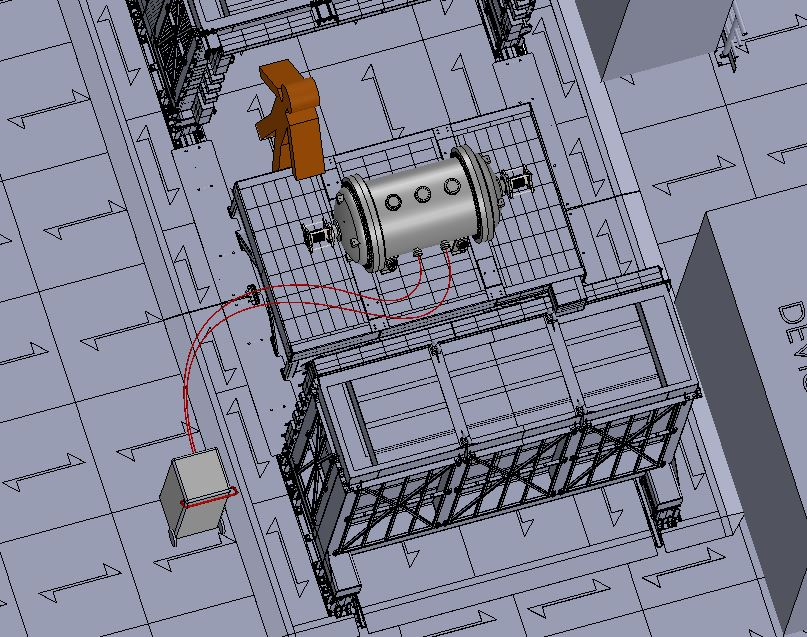
\includegraphics[width=0.6\textwidth]{img/CALIB_LSC_sources.jpg}
%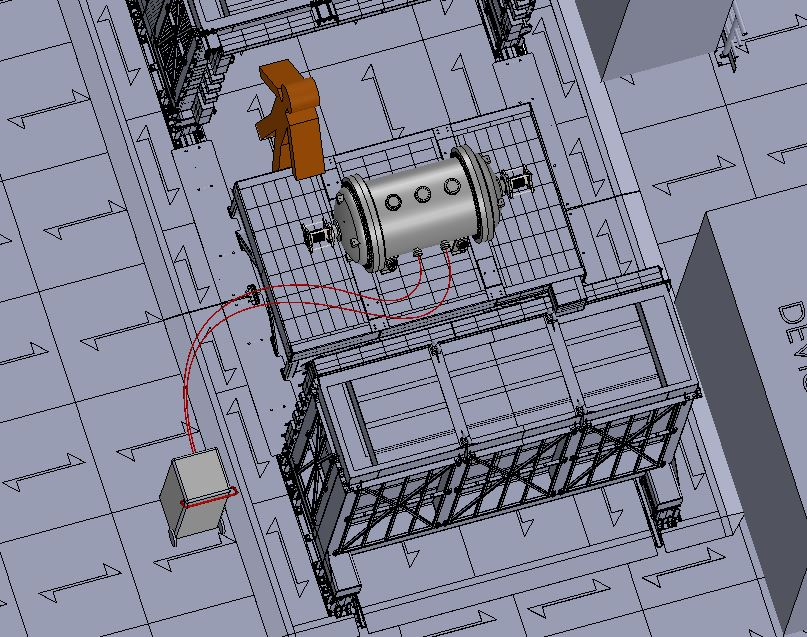
\includegraphics{img/CALIB_LSC_sources.jpg}
\caption{\small Drawing of the NEW detector at the LSC platform. The lead closet with the radioactive sources is on the left,  guides transmit gamas into the vessel via two ports on the side.}
\label{fig:CALREC_LSC_sources}
\end{center}
\end{figure}

To calibrate in energy, we will use several radiative sources.
\Tl ~emits a high energy gamma of 2.6 MeV and the double scape peak produces two electrons around 1.6 MeV energy.
The energy resolution and scale will be obtained from the width a position of the 2.6 MeV photo-peak, that is very close the \Qbb. 
From the two electrons at 1.6 MeV we can estimate the efficiency to identify a \bb signal.  
In addition to the \Tl, \NA ~(511 keV) and \CS ~(662 keV)  sources will be used to calibrate the energy scale around 500 keV. 
%The sources will be located inside a lead closet on the LSC platform outside the NEXT castle.
%two light guides will direct the gamma rays into the vessel via two ports located on the side. 
The sources will be located in a lead shielded closet outside the NEXT castle, a light guide will direct the gammas to the two ports (see Fig. ~\ref{fig:CALIB_LSC_sources}) on the side of the vessel. 
Calibration will take place before the start of the run in a periodic basis.
%The detector will be calibrated before we the start of the run and periodically.
%The Calibration procedure itself (security measures,
We are still defining the procedure for the calibration runs (security, time, periodicity and type). This calibration method has been previously used in other \bb experiments (see \cite{COURE-Tl}). We expect no difficulties. 
%A good communication with technical coordinator is essential.
%This part requires that the responsible of the calibration to be frequently at LSC.

{\bf Calibration in Position}

Position calibration is needed to correct for the bias on the energy introduced by the geometry of the chamber. According with the results from NEXT-DEMO (see \cite{NEXT-DEMO}) PMTs detect less light departing for events outside the central region of the detector. To correct for the geometrical dependence we will use X-rays from \Xe ~ (30 keV)  and \KR ~(42 keV). X-rays are point like sources for NEXT.
The correction to the bias can be obtained from the measurement of the X-ray energy as a function of $z$ and the position on the transverse plane $x,z$.
A large statistic sample is necessary to map the full vessel volume.
For that reason, we plan to introduce \KR with the \Xe gas to increase the number of X ray interactions.  \KR ~as a half-life of $1.83 \pm 0.02$ hours and
tt should leave no trace in few days. 
As it is a pure noble gas, it should not compromise the purity of xenon.
The details of the calibration (injection, rates, etc) with \KR~ are still to be defined.
Most probably NEW will be calibrated with \KR~ before each start of the run.
Nevertheless we will dedicate R+D efforts to test the injection system and study possible secondary effects (as electron attachment). NEXT-DEMO prototype could be reused for this propose. 
Successful examples using this calibration exits in other experiments (\cite{KR}), nevertheless, for contingency, we plan to explore other calibration sources. 

Notice also that X-rays could be used to estimate the Point Spread Function (PSF), that is the probability that light reach a given SiPM from a point-like source. We can study the PSF as a function of the position on the chamber. This function a key ingredient for the reconstruction. Algorithms to estimate the PSF from data need to be in place, but no difficulties are expected here.  
 
{\bf Reconstruction algorithms}

The reconstruction algorithms converts the calibrated signal from the SiPMs and PMTs into a 3D trajectory. Each point of the trajectory has associated a deposited energy. 
A trajectory is as an electron if a {\it blob} is found in one of the end-points of the trajectory. 
A \bb ~signal is therefore a trajectory with two blobs.
Algorithms are pieces of C++ code that runs in the official reconstruction program, inside a C++ framework.
Three algorithms are currently on place, they are in a primitive state, they run from simple to complex.
The simple one has been developed by the IFIC group for the NEXT-DEMO reconstruction \cite{NEXT-DEMO2}. A collection of SiPMs are clustered together if they meet a given criteria of proximity and signal threshold. These clusters are connected into a 3D trajectory and an interpolation is done between the different points. This method is simple and good enough for an initial reconstruction pass of all events. But it lacks the capability to find complex structures as twists in the transverse plane, two segments in the same $z$ location or vertical tracks. 
A second algorithm has been develop by the USC group. It used the signal collected by the SiPMs and the PSF to recover the image of the electron cloud at the EL using a Fast Fourier transform. The method is still in a preliminary stage, but it allows us to recover the transverse plane image. See for example in Fig.~\ref{fig:REC_FF}, that represents a muon candidate traversing vertically the NEXT-DEMO detector. Next step is to connect the transverse images into a 3D trajectory. This method is fast enough to process a large amount of data and provides the capability of finding complex structures in the transverse plane. 
Finally the third method, also in primitive stage, is been developed by the IFIC group. The full detector volume is divided in $5\times5\times5$ mm$^3$ 3D boxes. Using the probability function that associates the deposited energy in a given 3D box with the signal detected at the SiPMs and PMTs, and via an iterative process, the method finds the 3D trajectory that maximizes the likelihood that the detected signal match the image produced by the 3D trajectory. This is a time consuming algorithm but it expected to have the ultimate resolution. Notice nevertheless, that it relies on the accurate estimation of the signal left on the PMTs and SiPMs from a deposition at a given point of the detector. 

We will continue developing and improving these algorithms.
The final goal is to have the best reconstruction possible to be applied to the relevant events in the \Qbb ~region. 
Algorithms will be validated using simulated data, on computing time  and performance. 
Moreover, they will be validated with real data from the \NA,  ~\CS ~and \Tl ~sources. Similar studies are been carried out with the NEXT-DEMO data with \NA ~and ~\CS.
The definition of an algorithm requires an effort of success and failure trials to finally get the final version. It also requires a detailed comparison data/simulation and validation. This is intelectual challenge, there are no technological problems expected.

The algorithms to identify a blob will require the combination of tracking and energy measurements. Fig ~\ref{fig:REC_blob} shows the average energy profile for horizontal track moving towards the anode, obtained with NEXT-DEMO with \NA ~events. The mip and blob parts are clearly visible. This is on average, but event by event, there are large fluctuations and therefore a sophisticated selection needs to be defined. This will require the use of multivariate techniques and detailed studies of the blob structure with simulation and calibration data.
Therefore, the blob-selection algorithm requires validation.
Remember that the \Tl ~photo-peak signal (2.6 MeV) is a great candle to estimate the efficiency of the blob-identification algorithm. Furthermore, the double-peak scape (1.6 MeV) provides two electrons, that allow us to estimate the efficiency of identifying two blobs. 

{\bf \bb ~Analysis}

The measurement of \bb ~spectrum is a data analysis (including simulation samples) starting from reconstructed 3D trajectories.
The analysis uses software programs and techniques common on HEP.
It has several steps: definition of the signal region, estimation of the contamination events on that region, estimation of the signal yield, a fine study of the measurement uncertainties.
Large MC samples will be used to define the signal selection. Multi-Variate Technique (such as Neural Network or Boosted Decision Trees) will be used to separate the signal from the background.
The efficiency of the selection and the contamination levels will be estimated from data, using the \Tl ~two-electrons from the doble scape peak at ~1.6 MeV and the photo-peak at 2.6 MeV, as commented before. The energy scale and resolution will be estimated using the 2.6 MeV \Tl ~photo-peak. The expected energy spectrum of the detector will be obtained from the radio purity measurements in conjunction with the detector simulation. Uncertainties on the spectrum around the region of interest will be carefully estimated.
The yield of \bb~ events will be obtained from the fit and used to measure the life-time of this process. 
It has been already measured by EXO-200 \cite{EXO} and KamLAND-Zen \cite{KAMLAND}.
This measurement is a mayor milestone of the NEXT collaboration. 
It will confirm the capabilities of NEXT technique to detector a \bbonu signal and will provide an estimated, based on data, of the sensitivity to be obtain with NEXT-100 and NEXT 1 ton. 

The \bbonu search to be perform with NEXT-100 data is similar to the described above. The expected signal spectrum could be estimated from the famous \Tl ~2.6 MeV peak. 
Data will be fit to all contributions, including a possible \bbonu ~signal.
From the estimated yield and detection efficiency, we could them measure, or set a limit in, the life-time on the \bbonu decay.

{\bf R+D with gas mixture}

Within this project the USC will incorporate into the R+D of NEXT. 
NEXT collaboration pursues several R+D lines to improve the detector performance. 
The first one is the use of additives (for example TMVA, tre-methylamine) mixed with xenon.  These additives reduce the electron diffusion, which translate to a more confined trajectory.  In addition the scintillator light has  a 300 nm wavelength, easier to detect than the one of Xenon (170 nm). Preliminary results have been published by the NEXT collaboration \cite{NEXT-TMVA}. The R+D should be focus on the handling of the mixtures and the study of the detector performance as function of additive concentration and pressure. This studies could be done with the NEXT prototypes of UZ.
The second R+D line could result in an excellent synergy between \bb and dark matter detectors. Electrons from ionization produced by a nuclear recoil, could recombine different depending on the angle between the recoil and the electric field. As the dark matter should be a flux with a privileged direction, we could determine an excess on that direction (see \cite{NEXT-DM-1}). Preliminary studies at \cite{NEXT-DM} are promising. Further studies are needed to proof this detector concept. This R+D could be done in collaboration with the Berkeley group.
The third R+D line is the \BATA proposal, of tagging the Ba product of the \bbonu decay with lasers exploiting the convenient atomic levels. This is a challenging proposal to be carried out in collaboration in collaboration with the Center for Pulsed Lasers (CLPU) at Salamanca. 

 


